\section{Introduction}
This work explores the possibilities of decentralized video streaming using \ac{P2P} technologies. The main goal is to create a functional prototype of a \ac{P2P} video streaming application and evaluate its performance and stability. The motivation behind this work is to address the limitations of traditional centralized video streaming solutions such as expensive infrastructure costs, single points of failure, and scalability issues. By leveraging \ac{P2P} technologies, I aim to test the feasibility of a decentralized approach to video streaming that can potentially offer improved scalability, resilience, and cost-effectiveness. I will also explore downside of \ac{P2P} video streaming such as latency, quality and security concerns.

Taking into account outages of major centralized server providers, like AWS or Cloudflare, it is clear that there is need for more decentralized solutions that are not dependent on single entities. This work aims to contribute to the understanding of how \ac{P2P} technologies can be applied to video streaming and what benefits and challenges they bring.

The paper is structured into several parts. First, I will provide an overview of video recording and encoding techniques. Then, I will discuss the current state of video streaming and the challenges associated with it. Next, I will describe the implementation of the \ac{P2P} video streaming prototype, including the choice of programming language, screen recording, encoding, and transport layer. Finally, I will present the results of performance and stability testing and conclude with a summary of findings and future work.

\section{What is video streaming}
Video streaming is method of video data transmission from server to client. On surface level the video streaming consists of 3 main parts.
\begin{itemize}
    \item Producer - Creates video stream to be provided to consumers
    \item Transport layer - Provides provided video stream to all consumers
    \item Consumer - Accepts video stream from transport layer
\end{itemize}
These 3 parts can be implemented in various ways depending on the use case. The most common implementation is client-server model where producer and consumer are separate entities and transport layer is provided by central server or \ac{CDN}.

\subsection{Static video streaming}
Static video streaming is method of video streaming where the video content is pre-recorded and stored on a server. The server then delivers the video content to clients upon request. This method is commonly used for on-demand video services, such as Netflix or YouTube, where users can choose from a library of pre-recorded videos to watch at their convenience.

This method allows for efficient use of bandwidth and decrease of latency, as the video can be stored on \ac{CDN} located closer to the user.
\subsection{Live video streaming}
Live video streaming is method of video streaming where the video content is captured and transmitted in real-time. This means there is no video file but rather a continuous stream of video data being sent from the producer to the consumer.

According to Cloudflare \ac{CDN} can also be used to distribute the live stream to multiple viewers, but the latency is usually higher compared to static video streaming due to the real-time nature of the content. \cite{WhatVideoCDN}
\subsection{\ac{P2P} video streaming}
\ac{P2P} video streaming is method of video streaming where the video content is distributed among multiple peers in a decentralized manner. In this model, each peer can act as both a producer and a consumer of video content in the transport layer. This means that when a peer receives a video stream, it can also share that stream with other peers in the network, reducing the load on the original producer and improving scalability.
The clear downsides of \ac{P2P} video streaming are increased latency and potential quality issues due to the decentralized nature of the network. Additionally, security concerns may arise as peers may not be trustworthy sources of video content.

\section{Handling video streams}
Common stream sources for streaming are camera or computer screen. In raw form, these data sources are not viable for network transport due to their large sizes.

\begin{itemize}
    \item "A single frame of high definition (1920x1080) video in full color (4 bytes per pixel) is 8,294,400 bytes." \cite{WebVideoCodec2025}
    \item "At a typical 30 frames per second, each second of HD video would occupy 248,832,000 bytes (~249 MB)." \cite{WebVideoCodec2025}
    \item "A minute of HD video would need 14.93 GB of storage." \cite{WebVideoCodec2025}
    \item "A fairly typical 30 minute video conference would need about 447.9 GB of storage, and a 2-hour movie would take almost 1.79 TB (that is, 1790 GB)." \cite{WebVideoCodec2025}
\end{itemize}

The prepending calculation describes the size of raw video stream that we can get from source like screen recording. Because of that we need to first encode these streams into more effitient format.

For that we use a video codec, which handles the problem of large video files, by encoding video into more predictive patterns, decreasing overall size of the stream.
It is decreasing entropy of the video stream and removing redundant information.

\subsection{Video codec}
Video codec is software that compresses and decompresses digital video. The term "codec" is a portmanteau of "coder-decoder" or "compressor-decompressor." Video codecs are essential for reducing the size of video files, making them easier to store and transmit over networks.

All video codecs work by optimizing the representation of video data and therefore reducing entropy of the video stream.

"As is the case with any encoder, there are two basic groups of factors affecting the size and quality of the encoded video: specifics about the source video's format and contents, and the characteristics and configuration of the codec used while encoding the video." \cite{WebVideoCodec2025}

\break
Smaller video sizes often require more destructive approach to reducing entropy of video stream or more computing power, usually both. It is important to balance these three parameters when choosing codecs and their configurations.

List of commonly used codecs and their characteristics:
\begin{itemize}
    \item AV1
    \begin{itemize}
        \item 50\% better compression than H264 \cite{WebVideoCodec2025}
        \item Slow encoding speed
        \item Limited hardware support \cite{WebVideoCodec2025}
        \item "Royalty-free, open standard" \cite{WebVideoCodec2025}
    \end{itemize}
    \item H264
    \begin{itemize}
        \item Baseline compression
        \item Fast encoding
        \item Full hardware and software support \cite{WebVideoCodec2025}
        \item "Proprietary with numerous patents. Commercial use requires a license." \cite{WebVideoCodec2025}
    \end{itemize}
    \item H265
    \begin{itemize}
        \item 50\% better compression than H264 \cite{WebVideoCodec2025}
        \item Slower encoding speed
        \item Mostly full hadrware and software support \cite{WebVideoCodec2025}
        \item "Proprietary; confirm your compliance with the licensing requirements." \cite{WebVideoCodec2025}
    \end{itemize}
    \item VP8
    \begin{itemize}
        \item Similiar compression to H264
        \item Fast encoding speed
        \item Full hardware and software support \cite{WebVideoCodec2025}
        \item "Open and free of royalties and any other licensing requirements" \cite{WebVideoCodec2025}
    \end{itemize}
    \item VP9
    \begin{itemize}
        \item 50\% better compression than H264 \cite{WebVideoCodec2025}
        \item Normal encoding speed
        \item Full hardware and software support \cite{WebVideoCodec2025}
        \item "Open and free of royalties and any other licensing requirements" \cite{WebVideoCodec2025}
    \end{itemize}
\end{itemize}

\subsection{Muxers}
After the video and audio have been separately compressed by their respective codecs, they need to be combined into a single, synchronized package for delivery. This process is called multiplexing, or muxing.

A muxer interleaves the compressed video and audio streams (along with any other data, like subtitles or chapter markers) into a single file or stream, known as a container format. The container file includes timing information and metadata that tells the consumer's video player how to synchronize the different streams so that the audio perfectly matches the video playback.

\section{Current state of video streaming}
\subsection{Video streaming in video calls}
Video calls are a common use case for real-time video streaming. Popular applications like Zoom, Microsoft Teams, and Google Meet utilize centralized servers to manage video streams between participants. These applications use centralized servers to handle video distribution, which incurs cost and scalability issues.
\subsection{Video streaming in live streaming}
Live streaming platforms like Twitch, YouTube Live, and Facebook Live also rely on centralized servers and \ac{CDN}s to distribute live video content to viewers. Content creators depend on these platrofms to reach their audience, but they are subject to the platforms policies and potential outages.
\subsubsection{Possibility of censorship}
Centralized platforms have the authority to censor content based on their policies, which can limit freedom of expression for content creators. Decentralized \ac{P2P} video streaming could potentially mitigate this issue by distributing control among multiple peers.
\subsection{Existing \ac{P2P} video streaming solutions}
There is an existing \ac{P2P} solution like P2P Media Loader \cite{NovageP2pmedialoader2025} which uses hybrid approach, combining \ac{P2P} technologies with centralized servers to optimize performance and reliability.
There is also IPFS which offers static video storage and streaming capabilities using its decentralized file system. However, IPFS does not support real-time live video streaming.



\section{Implementation of \ac{P2P} video streaming}
\subsection{Choice of programming language}
I have chosen Rust programming language because of my familiarity with programming in the chosen language but alse because of it's speed. Fast programming language is needed for critical systems like video streaming.
\subsection{Screen Recording}
For screen recording I have chosen to only implement wayland screen capture, as that is the platform I am developing on and it also abstracts any need for handling window and screen choice. That is handled on the OS side.
I am using 
\subsection{Encoding}
There are 2 main encoding/decoding libraries. FFmpeg and GStreamer.
\subsubsection{Gstreamer}
GStreamer is a pipeline-based framework. You build a graph of processing elements to manage the flow of media. It is highly modular and flexible, ideal for complex, dynamic media applications.
\subsubsection{FFmpeg}
FFmpeg is a collection of libraries for encoding. There 
\subsection{Network Layer}

\subsubsection{Security}
\subsubsection{Authentication}
\subsection{Gossipsub}

\subsection{Stream}
\subsubsection{Integrity check}
\subsection{Combination of Gossipsub and Stream}
\section{Current implementation}
My implementation is split into my testing binary I am using to glue all the parts together and then library crates for screen recording, decoding and transport layer.
\subsection{Screen recording crate}
For screen recording I am using ashpd's wayland-capture library. It provides simple interface for capturing screen content on wayland compositors supporting the screen-capture portal. This portal is already widely supported by most wayland compositors including major compositors like GNOME's Mutter and KDE's KWin.
Using the library I receive pipewire file descriptor which I then provide to GStreamer's pipewire source element to get video frames into GStreamer pipeline.

\begin{figure}[h]
    \centering
    \includegraphics[width=1\textwidth]{out/recorder-pipeline/recorder-pipeline.png}
    \caption{Recorder pipeline}
\end{figure}

The Recorder Pipeline displays the flow of data from the PipeWire source to the final encoded video stream. It starts with capturing video frames from the PipeWire source, processes them through various elements like videorate, videoconvert, and x264enc for encoding, and finally packages them into RTP packets for transmission.

There are also edge cases for when hardware encoding is unavailable, in which case software encoding is used instead. The final output is an RTP stream that can be sent over the network. The benefit of encoding into RTP packets is their consistent size, which prevents sending large packets that could clog the transport layer. The output of the pipeline is then sent into the memory of host program to be then used in the transport layer.

\break
\subsection{Rendering crate}
For decoding I am also using GStreamer. The decoding pipeline is much simpler than the encoding pipeline as it only needs to decode the incoming RTP packets back into raw video frames for display.

\begin{figure}[h]
    \centering
    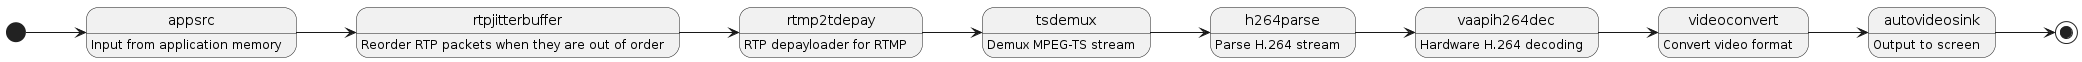
\includegraphics[width=1\textwidth]{out/renderer-pipeline/renderer-pipeline.png}
    \caption{Recorder pipeline}
\end{figure}

The decoding pipeline consists of RTP depayloader, H264 decoder, videoconvert, and autovideosink elements. The RTP depayloader extracts the encoded video data from the RTP packets, which is then decoded by the H264 decoder. The videoconvert element ensures that the video format is compatible with the display sink, which is handled by autovideosink.

\subsection{Transport layer crate}
The transport layer is implemented using libp2p's Gossipsub protocol for peer-to-peer communication.

There are two implementations of the transport layer. The first one uses only Gossipsub for sending video data, while the second uses solely stream to send data between peers. Finally, there is a hybrid implementation that combines both Gossipsub and stream for data transmission.
\subsubsection{Gossipsub}

\subsubsection{Stream}
\subsubsection{Hybrid}

\section{Testing of stability and performance}
\subsection{Latency testing}
\subsection{Packet order variability}
\subsection{Late packet testing}
\subsection{Throughput testing}

\section{Conclusion}